
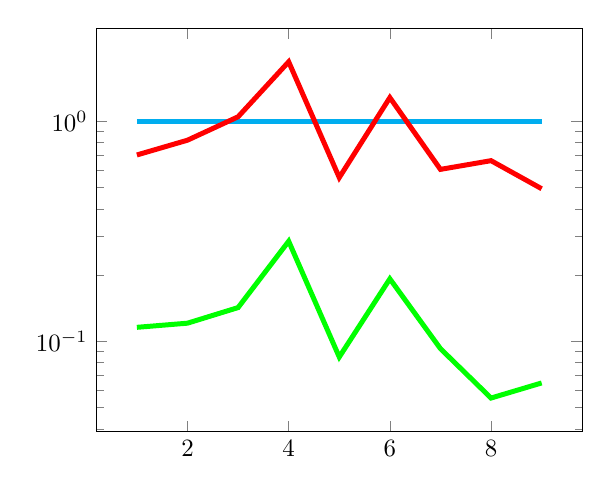
\begin{tikzpicture}[scale=0.9]
\begin{semilogyaxis}
\addplot[color=cyan,line width=2pt] coordinates {(1,1.0)(2,1.0)(3,1.0)(4,1.0)(5,1.0)(6,1.0)(7,1.0)(8,1.0)(9,1.0)};
\addplot[color=red,line width=2pt] coordinates {(1,0.7034754472025413)(2,0.8210112334915415)(3,1.048998782033453)(4,1.8659386573616588)(5,0.5552362722508278)(6,1.2825633870888684)(7,0.6049422257015237)(8,0.6626399086954456)(9,0.49384647952196853)};
\addplot[color=green,line width=2pt] coordinates {(1,0.1157078684163629)(2,0.12085102576740576)(3,0.14229324653411546)(4,0.2849918180729477)(5,0.08479366411486086)(6,0.1922611619637746)(7,0.09254905053749439)(8,0.055186558737763416)(9,0.0646357214690336)};

\end{semilogyaxis}
\end{tikzpicture}
